\documentclass{article}
\usepackage{amsmath}

\usepackage{full page}  % make the margins somewhat smaller than the default

\usepackage{listings}  %  needed for source code listings
\usepackage{color}
\usepackage{hyperref}
\usepackage{graphicx}
\usepackage{caption}
\usepackage{subcaption}
\usepackage{float}

\graphicspath{ {images/} }

\definecolor{javared}{rgb}{0.7,0,0} % for strings
\definecolor{javagreen}{rgb}{0.25,0.6,0.35} % comments
\definecolor{javapurple}{rgb}{0.55,0,0.40} % keywords
\definecolor{javadocblue}{rgb}{0.25,0.35,0.85} % javadoc
 
\lstset{language=Java,
basicstyle=\ttfamily,
keywordstyle=\color{javapurple}\bfseries,
stringstyle=\color{javared},
commentstyle=\color{javagreen},
morecomment=[s][\color{javadocblue}]{/**}{*/},
numbers=left,
numberstyle=\tiny\color{black},
stepnumber=2,
numbersep=10pt,
tabsize=2,
showspaces=false,
showstringspaces=false,
frame=shadowbox,
numbers=left
} 

% set the document title, author, and date here.
%  once set, the \maketitle command (within the document)
%  will display them nicely
\title{AI Assignment 6 - HMM and First Order Logic}
\author{Tianyuan Zhang}

\begin{document}
\maketitle

\section{Introduction}
The probabilistic reasoning is an important topic in AI field. Given the initial states, the states transformation, and the evidence, we can compute the probability of each state in each step. In this assignment, we focus our attention on a specific problem - evaluating the position of a robot in a maze. We are given a 4x4 maze. Each position of the maze has one of the four colors. The maze may contain obstacles. Also, a series of colors that read by the robot sensor are given. Our purpose is to figure out the most likely position of the robot after each move. Note that the there is a chance that the color read by the robot is wrong. From the state transform and evidence, we can compute the probability distribution at each step.

\section{Filtering Method}
The method used here is the filtering described in the book and class. Suppose $X_t$ represents the probability of the robot in position $X$ in time $t$, then with filtering, we can compute $P(X_t|e_{1:t})$ based on the previous distribution and the current evidence $e_t$. 
\subsection{Transition Model}
The transition model is quite straightforward for this problem. In each time step $t$, for a position $X$, the only possible move from the previous step is from north, south, east or west position in time $t-1$, and the only possible move to the next step would be to north, south, east or west. The probability of a robot moving to each direction is the same.If any of the position is invalid, either out of bound or facing an obstacle, then the robot will simply not move and the probability to move to that direction will be assigned to the current position. The following is an example considering only one position in the maze. 
\begin{figure}[H]
\centering
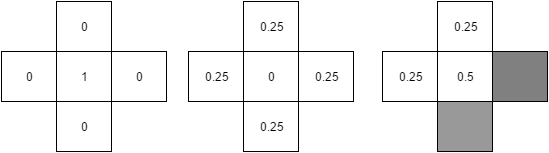
\includegraphics[width=0.7\linewidth]{transition_model}
\caption{Transition Model}
\medskip
\small
Assume that we know that the robot is in the middle position at the beginning. After one move, the chance for the robot to move in each direction is 25\%. However as shown in the right most graph, if two of the directions are invalid, then the robot still have 50\% of chance that stay in the same position.
\end{figure}

\section{Sensor Model}
After we predict in each step, we need to take the evidence we learned in current step into consideration.Given the probability the robot is at position X in time t and given the current color read from the sensor, if the read color matches the color in position X, there is a large probability that robot may in position X. And as for this problem, the correctness of the sensor is 88\% and chance to read the rest of colors is 4\% each, we can simply multiply 0.88 to those positions that match the read color and 0.04 to those positions that don't match. The following figure shows the sensor model.
\begin{figure}[H]
\centering
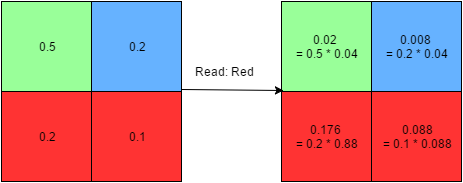
\includegraphics[width=0.7\linewidth]{sensor_model}
\caption{Sensor Model}
\medskip
\small
The left is the probability after prediction and the right is the probability after considering evidence.
\end{figure}

\section{Implementation}
Though this assignment is based on the maze, it quite different from what we have done before and it turns out that I rewrite a new one to make the code simply and clear. The class $MazeWorld$ is for constructing the maze and the class $ProbReasoning$ and $ProbReasoningDriver$ is for solving the probabilistic reasoning problem. All the methods and class that solve the probabilistic problem is in the class $ProbReasoning$ and I will mainly introduce the methods and subclass in $ProbReasoning$ class.

\subsection{members}
Here are the members used to solve the probablistic reasoning problem.
\begin{lstlisting}
	//Store the maze
	private MazeWorld maze;
	//Store the distribution of each step
	private HashMap<Integer, HashMap<Coor, Double>> distributions;
	//Store the valid position in the maze
	private HashSet<Coor> validPos;
	//Store the color read by the sensor
	private String colorsRead;
	//Store how many positions are valid
	private int validPosNum;
\end{lstlisting}
\subsection{Coor}
This subclass is for storing and hashing the coordinate of the maze.
\begin{lstlisting}
	public class Coor {
		protected int x;
		protected int y;

		public Coor(int _x, int _y) {
			x = _x;
			y = _y;
		}

		@Override
		public boolean equals(Object other) {
			return this.x == ((Coor) (other)).x && this.y == ((Coor) (other)).y;
		}

		@Override
		public int hashCode() {
			return x * 37 + y;
		}

		@Override
		public String toString(){
			return "[" + Integer.toString(x) + "," + Integer.toString(y) + "]";
		}
	}
\end{lstlisting}

\subsection{predict}
The method $predict$ takes the time step as the input and use the transition model described above to estimate the next distribution for each of the valid position in the maze. The update method needs to be called to complete the whole estimation.
\begin{lstlisting}
	public void predict(int curStep) {
		distributions.put(curStep, new HashMap<>());
		if (curStep == 0) {
			for (Coor coor : validPos) {
				Coor curCoor = new Coor(coor.x, coor.y);
				distributions.get(curStep).put(curCoor, 1.0 / validPosNum);
			}
		} else {
			HashMap<Coor, Double> preDistr = distributions.get(curStep - 1);
			for (Coor coor : validPos) {
				Coor curCoor = new Coor(coor.x, coor.y);
				double curCoorDistr = getCurCoorDistr(curCoor, preDistr);
				distributions.get(curStep).put(curCoor, curCoorDistr);
			}
		}
		update(curStep);
		normalize(curStep);
	}
\end{lstlisting}

\subsection{getCurCoorDistr}
This is a method that called by the $predict$ method. It takes the current estimating coordinate and the previous distribution as the input, returns the distribution for the estimating position.
\begin{lstlisting}
	private double getCurCoorDistr(Coor curCoor, 
			HashMap<Coor, Double> preDistr) {
		int[] dir = { 0, 1, 0, -1, 0 };
		double res = 0;
		double inValidAdjPos = 0;
		for (int i = 0; i < dir.length - 1; i++) {
			Coor adjCoor = new Coor(curCoor.x + dir[i], curCoor.y + dir[i + 1]);
			if (validPos.contains(adjCoor)) 
				res += preDistr.get(adjCoor) * 0.25;
			else inValidAdjPos++;
		}
		res += preDistr.get(curCoor) * inValidAdjPos * 0.25;
		return res;
	}
\end{lstlisting}

\subsection{update}
This is a method that update the distribution according to the evidence read in the current time step using the sensor model described above.
\begin{lstlisting}
	private void update(int curStep) {
		char curReadColor = colorsRead.charAt(curStep);
		for (Coor coor : validPos) {
			char coorColor = maze.getColor(coor.x, coor.y);
			double updateDistr = distributions.get(curStep).get(coor);
			if (coorColor == curReadColor)
				updateDistr *= 0.88;
			else
				updateDistr *= 0.04;
			distributions.get(curStep).put(coor, updateDistr);
		}
	}
\end{lstlisting}

\subsection{normalize}
This is a method that normalizes the distribution.
\begin{lstlisting}
	private void normalize(int curStep) {
		HashMap<Coor, Double> curDistribution = distributions.get(curStep);
		double totalSum = 0;
		for (Coor coor : validPos) {
			totalSum += curDistribution.get(coor);
		}
		for (Coor coor : validPos) {
			double curCoorDistr = curDistribution.get(coor);
			curCoorDistr /= totalSum;
			curDistribution.put(coor, curCoorDistr);
		}
	}
\end{lstlisting}

\section{Result}
In the testing part I test two cases - 2x2 maze and a 4x4 maze. Each of them shows me reasonable result. 
\subsection{2x2 maze}
The Maze:
\begin{lstlisting}
RG
RG


\end{lstlisting}

The Path ('+' indicates the positions that have been visited)
\begin{lstlisting}
.+
++

Real Path Color: RGG
Color Read: RGG
\end{lstlisting}



The probability distribution
\begin{lstlisting}
Step: 0
[0,0] 0.47826086956521735
[0,1] 0.021739130434782608
[1,0] 0.47826086956521735
[1,1] 0.021739130434782608
Step: 1
[0,0] 0.05429497568881685
[0,1] 0.44570502431118314
[1,0] 0.05429497568881685
[1,1] 0.44570502431118314
Step: 2
[0,0] 0.009746917585983127
[0,1] 0.4902530824140168
[1,0] 0.009746917585983127
[1,1] 0.4902530824140168
\end{lstlisting}
From the result we can see that the two position with color Red have the highest posibility as the first read is red. Then in step 1 two position that have Green color have the highest posibility. 

\subsection{4x4 maze}
In this larger scale sample. Need to point out that the color read does not correspond to the actual path color, which may effect the estimation a bit. We can see that the step 0 and step 1 shows some kinds of wrong probability as the first two colors read are wrong. Then from step 2 to step 7 the distribution reflect the actual path more and more precisely as we got the right color read. For step 7, we can see that the position [0, 3] has the probability ~0.4, which is much higher than the other position and match the real path.

The Maze:
\begin{lstlisting}
RGYB
BGYY
RYBG
YGBG
\end{lstlisting}

The Path ('+' indicates the positions that have been visited)
\begin{lstlisting}
...+
...+
...+
++++

Real Path Color: YGBGGYB
Color Read: RYBGGYB
\end{lstlisting}



The probability distribution
\begin{lstlisting}
Step: 0
[0,0] 0.3793103448275862
[0,1] 0.017241379310344827
[0,2] 0.017241379310344827
[0,3] 0.017241379310344827
[1,0] 0.017241379310344827
[1,1] 0.017241379310344827
[1,2] 0.017241379310344827
[1,3] 0.017241379310344827
[2,0] 0.3793103448275862
[2,1] 0.017241379310344827
[2,2] 0.017241379310344827
[2,3] 0.017241379310344827
[3,0] 0.017241379310344827
[3,1] 0.017241379310344827
[3,2] 0.017241379310344827
[3,3] 0.017241379310344827
Step: 1
[0,0] 0.02998696219035201
[0,1] 0.01629726205997392
[0,2] 0.057366362451108203
[0,3] 0.0026075619295958274
[1,0] 0.02998696219035201
[1,1] 0.0026075619295958274
[1,2] 0.057366362451108203
[1,3] 0.057366362451108203
[2,0] 0.01629726205997392
[2,1] 0.3585397653194263
[2,2] 0.0026075619295958274
[2,3] 0.0026075619295958274
[3,0] 0.3585397653194263
[3,1] 0.0026075619295958274
[3,2] 0.0026075619295958274
[3,3] 0.0026075619295958274
Step: 2
[0,0] 0.006164202246341185
[0,1] 0.006164202246341186
[0,2] 0.007752524297545664
[0,3] 0.15308399198275535
[1,0] 0.10066936429300759
[1,1] 0.026812388911999396
[1,2] 0.006958363271943426
[1,3] 0.006958363271943426
[2,0] 0.04428393147524865
[2,1] 0.001399236092727754
[2,2] 0.5374579283742389
[2,3] 0.00378171916953447
[3,0] 0.04269560942404417
[3,1] 0.04190144839844193
[3,2] 0.013311651476761334
[3,3] 6.050750671255152E-4
Step: 3
[0,0] 0.005568712003393186
[0,1] 0.04821150855365474
[0,2] 0.008129506574296622
[0,3] 0.014995405061501484
[1,0] 0.008315071398275132
[1,1] 0.11842923794712286
[1,2] 0.02705711862010463
[1,3] 0.007981054715113813
[2,0] 0.008834652905414957
[2,1] 0.0303972854517178
[2,2] 0.0011893821575003534
[2,3] 0.5642301710730949
[3,0] 0.008018167679909517
[3,1] 0.10209953343701399
[3,2] 0.027725151986427263
[3,3] 0.018818040435458788
Step: 4
[0,0] 0.0017185917449781677
[0,1] 0.10076907732446412
[0,2] 0.0024990883433452476
[0,3] 0.001170924445882427
[1,0] 0.0035849966541168362
[1,1] 0.0636898331295759
[1,2] 0.003447372857786409
[1,3] 0.015601627856995499
[2,0] 0.00141129477508968
[2,1] 0.005855789293568883
[2,2] 0.0164942972756593
[2,3] 0.33091754045358573
[3,0] 0.003224912474676952
[3,1] 0.09400854398691738
[3,2] 0.0038055717797423156
[3,3] 0.3518005376036151
Step: 5
[0,0] 0.0050064608378707605
[0,1] 0.00783433429248558
[0,2] 0.11023942032716913
[0,3] 9.4947312020294E-4
[1,0] 0.003270009676610942
[1,1] 0.005278911434828046
[1,2] 0.10042839683795944
[1,3] 0.35879562271588883
[2,0] 6.538184711184874E-4
[2,1] 0.17943381620792073
[2,2] 0.015978606339277824
[2,3] 0.03320017223452657
[3,0] 0.1040913972630001
[3,1] 0.004964824887733146
[3,2] 0.02164884483577934
[3,3] 0.04822589051762803
Step: 6
[0,0] 9.132136360155374E-4
[0,1] 0.005550875144377382
[0,2] 0.009490159350209852
[0,3] 0.4480406532748031
[1,0] 0.013518453931447448
[1,1] 0.012582814080170507
[1,2] 0.021202643358547626
[1,3] 0.021335885337769034
[2,0] 0.012430699546080481
[2,1] 0.0011622563850432553
[2,2] 0.3184400396069155
[2,3] 0.0197283272483978
[3,0] 0.009245817700072458
[3,1] 0.013411919040807173
[3,2] 0.08640325737758188
[3,3] 0.006542984981761007

\end{lstlisting}

\section{First Order Logic}
For disk a and disk b, if the size of the disk a is greater than disk b than either disk b is on the top of the disk an or they are not in the same pillar.

$$\forall a, b (greater(size(a), size(b)) \wedge  (onTop(b, a)  |  \neg samePillar(a, b)))$$

The goal situation is that all the disks are in the same pillar while they are in right order

$$\forall a, b (greater(size(a), size(b)) \wedge  onTop(b, a)  \wedge  samePillar(a, b))$$

The rule to make move is that the moving disk must be on the top of its pillar and the pillar it is moving to must has a disk that has a large size on the top

$$\forall a (moving(a) \wedge topOfPillar(a) \wedge \exists b (topOfPillar(b) \wedge greater(size(b), size(a))))$$

\end{document}